\section{Optimal polynomial--wise constraint ratio}
\subsection{Inf--sup condition and its eigenvalue problem}

To ensure surjectivity of othogonal projection and the result's accuracy, the approximations of Eq.\eqref{mix_formulation} should satisfy the inf-sup condition, also known as the Ladyzhenskaya–Babuška–Brezzi condition \cite{bathe1996}:
\begin{equation}\label{infsup}
    \inf_{q_h \in Q_h} \sup_{\boldsymbol v_h \in V_h} \frac{\vert b(q_h,\boldsymbol v_h) \vert}{\Vert q_h \Vert_Q \Vert \boldsymbol v_h \Vert_V} \ge \beta > 0
\end{equation}
in which $\beta$, namely inf-sup value, is a constant independent of characterized element size $h$.
The norms of $\Vert \bullet \Vert_V$ and $\Vert \bullet \Vert_Q$ can be flexibly defined by:
\begin{align}
    \label{norm_V}
    \Vert \boldsymbol v\Vert_V^2 &= \int_\Omega \nabla^s \boldsymbol v : \nabla^s \boldsymbol v d\Omega \\
    \label{norm_Q}
    \Vert q \Vert_Q^2 &= \int_\Omega \frac{1}{3\kappa}q^2 d\Omega
\end{align}

% To further development of $\beta$'s estimator, we define the operator $\mathcal P = 3\kappa\nabla \cdot$ and 
% its the orthogonal projection operator $\mathcal P_h: V_h \rightarrow Q_h$, yields:
% \begin{equation}\label{Ph}
%     (q_h, \mathcal P \boldsymbol v_h) = (q_h, \mathcal P_h \boldsymbol v_h), \quad \forall q_h \in Q_h
% \end{equation}
% where $(\bullet,\bullet)$ is inner product operator.

\begin{lma}\label{lma}
Suppose $\mathcal P_h:V_h \rightarrow Q_h$ is the orthogonal projection operator of divergence operator $\mathcal P := 3\kappa \nabla \cdot$, i.e. $\mathcal P_h:= 3\kappa \tilde \nabla \cdot$ and satisfied Eq. \eqref{orthogonal}.
Such that the inf-sup value can be estimated by:
\begin{equation}\label{r1}
    \beta \le \inf_{V'_h \subset V_h \setminus \ker \mathcal P_h} \sup_{v_h \in V'_h} \frac{\Vert \mathcal P_h \boldsymbol v_h \Vert_Q}{\Vert \boldsymbol v_h \Vert_V}
\end{equation}
    in which $\ker \mathcal P_h \subset V$ is the kernel of $\mathcal P_h$ defined by $\ker \mathcal P_h := \{ \boldsymbol v \in V \;\vert\; \mathcal P_h \boldsymbol v = 0 \}$.
\end{lma}
\begin{pf}
As the definition of  $\mathcal P_h$, $\mathrm{Im}\mathcal P_h \in Q_h$, the Eq. \eqref{infsup} can be rewritten as:
\begin{equation} \label{r11}
\begin{split}
    \beta &\le \inf_{q_h \in Q_h} \sup_{\boldsymbol v_h \in V_h} \frac{\vert b(q_h,\boldsymbol v_h) \vert}{\Vert q_h \Vert_Q \Vert \boldsymbol v_h \Vert_V} 
    = \inf_{q_h \in Q_h} \sup_{\boldsymbol v_h \in V_h} \frac{\vert (q_h,\frac{1}{3\kappa}\mathcal P \boldsymbol v_h) \vert}{\Vert q_h \Vert_Q \Vert \boldsymbol v_h \Vert_V} \\
    &\le \inf_{q_h \in \mathrm{Im} \mathcal P_h} \sup_{\boldsymbol v_h \in V_h} \frac{\vert \frac{1}{3\kappa}(q_h,\mathcal P_h \boldsymbol v_h) \vert}{\Vert q_h \Vert_Q \Vert \boldsymbol v_h \Vert_V} 
\end{split}
\end{equation}

For a given $q_h\in \mathrm{Im}\mathcal P_h$, suppose a space $V'_h \subseteq V_h\setminus \ker P_h$ defined by:
\begin{equation}
    V'_h = \{ \boldsymbol v_h \in V_h \; \vert \; \mathcal P_h \boldsymbol v_h = q_h \}
\end{equation}
Since $\mathrm{Im}\mathcal P_h \in Q_h$, in accordance with Cauchy-Schwarz inequality, we have:
\begin{equation}
    \left \vert \frac{1}{3\kappa}(q_h,\mathcal P_h \boldsymbol v_h) \right \vert \le \Vert q_h \Vert_Q \Vert \mathcal P_h \boldsymbol v_h \Vert_Q
\end{equation}
where this equality is holding if and only if $q_h=\mathcal P_h \boldsymbol v_h$, i.e.,
\begin{equation}
    \left \vert \frac{1}{3\kappa} (q_h,\mathcal P_h \boldsymbol v_h) \right \vert = \Vert q_h \Vert_Q \Vert \mathcal P_h \boldsymbol v_h \Vert_Q, \quad \forall \boldsymbol v_h \in V'_h
\end{equation}
And the following relationship can be evidenced:
\begin{equation}\label{r12}
    % \begin{split}
        \sup_{\boldsymbol v_h\in V_h} \frac{\left \vert \frac{1}{3\kappa}(q_h,\mathcal P_h \boldsymbol v_h) \right \vert}{\Vert q_h \Vert_Q \Vert \boldsymbol v_h \Vert_V} =
        % \sup_{\boldsymbol v_h\in V'_h} \frac{\Vert q_h \Vert_Q \Vert \mathcal P_h \boldsymbol v_h \Vert_Q}{\Vert q_h \Vert_Q \Vert \boldsymbol v_h \Vert_V} \\ &=
        \sup_{\boldsymbol v_h\in V'_h} \frac{\Vert \mathcal P_h \boldsymbol v_h \Vert_Q}{\Vert \boldsymbol v_h \Vert_V}
    % \end{split}
    ,\quad \forall q_h \in \mathrm{Im}\mathcal P_h
\end{equation}

Consequently, with a combination of Eqs. \eqref{r11} and \eqref{r12}, Eq. \eqref{r1} can be obtained.
\end{pf}

\begin{rmk}
With Lemma \ref{lma} and the norm definitions in Eqs. \eqref{norm_V},\eqref{norm_Q}, 
the square of inf--sup value can further bounded by:
\begin{equation}
    \beta^2 \le \inf_{V'_h \subset V_h \setminus \ker \mathcal P_h} \sup_{v_h \in V'_h} \frac{\Vert \mathcal P_h \boldsymbol v_h \Vert_Q^2}{\Vert \boldsymbol v_h \Vert_V^2} =
    \inf_{V'_h \subset V_h \setminus \ker \mathcal P_h} \sup_{v_h \in V'_h} \frac{\tilde a(\boldsymbol v_h, \boldsymbol v_h)}{a(\boldsymbol v_h, \boldsymbol v_h)}
\end{equation}
The left hand side of above equation is consistance with the minimum-maximum principle \cite{babuska1991a}
and again proof the equivalence with traditional numerical inf-sup test \cite{malkus1981}. 
Since that, $\beta^2$ evaluates the non-zero general eigenvalue of $\tilde a$ and $a$ in Eq. \eqref{weak_penalty}.
\end{rmk}

\subsection{Inf--sup value estimator}

% In order to further figure out the optimal constraint counting ,

\begin{thm}
    Suppose that $P_{n_u}$ is a polynomial space with $n_u$ dimensions, and $V_{n_u}$ is the polynomial displacement space, $V_{n_u} = P_{n_u}^{n_d}$. The optimal dofs of pressure $n_p$ is equal to $n_c = \dim(V_{n_c}\setminus \ker \mathcal P)$.
    \begin{equation}\label{estimator}
        \beta \le \beta_s + Ch 
    \end{equation}
    with
    \begin{equation}\label{beta_s}
        \beta_s = 
        \inf_{V' \subset V_{n_u} \setminus \ker \mathcal P_h \mathcal I_h} \sup_{v \in V'} \frac{\Vert \mathcal P \boldsymbol v \Vert_Q}{\Vert \boldsymbol v \Vert_V}
    \end{equation}
\end{thm}
\begin{pf}
    As the dimensions of $V_h$ and $V_{n_u}$ is identical, $\dim V_{n_u}=\dim V_h = n_d\times n_u$. There exists a unique $\boldsymbol v \in V_{n_u}$ satisfing $\boldsymbol v_h = \mathcal I_h \boldsymbol v$. And the right side of Eq. \eqref{r1} becomes:
\begin{equation}\label{r21}
\inf_{V'_h \subset V_h\setminus \ker \mathcal P_h}\sup_{\boldsymbol v_h \in V_h'} \frac{\Vert \mathcal P_h \boldsymbol v_h \Vert_Q}{\Vert \boldsymbol v_h \Vert_V} = 
\inf_{V'\subset V_{n_u}\setminus \ker \mathcal P_h \mathcal I_h}\sup_{\boldsymbol v \in V'} \frac{\Vert \mathcal P_h \mathcal I_h \boldsymbol v \Vert_Q}{\Vert \mathcal I_h \boldsymbol v \Vert_V}
\end{equation}

In accordance with triangular inequality, Cauchy-Schwarz inequality and the relationship of Eqs. \eqref{Ph}, we have:
\begin{equation}\label{interpolation1}
\begin{aligned}
    \Vert \mathcal P_h \mathcal I_h \boldsymbol v \Vert_Q &= 
    \sup_{q_h \in Q_h} \frac{\left \vert \frac{1}{3\kappa}(q_h, \mathcal P_h \mathcal I_h \boldsymbol v) \right \vert}{\Vert q_h \Vert_Q}
    =\sup_{q_h \in Q_h} \frac{\vert (q_h, \mathcal P \mathcal I_h \boldsymbol v) \vert}{\Vert q_h \Vert_Q} 
    % & \text{Eq. \eqref{Ph}}
    \\
    &\le \sup_{q_h \in Q_h} \frac{\vert (q_h, \mathcal P \boldsymbol v)\vert + \vert (q_h, \mathcal P \boldsymbol v - \mathcal P \mathcal I_h \boldsymbol v) \vert}{\Vert q_h \Vert_Q} 
    % & \text{Triangular inequality}
    \\
    &\le \Vert \mathcal P \boldsymbol v \Vert_Q
    + \Vert \mathcal P(\mathcal I - \mathcal I_h) \boldsymbol v \Vert_Q \\
\end{aligned}
\end{equation}
Obviously, the second and third terms on the right side of Eq. \eqref{interpolation1} are the interpolation error and the orthogonal projection error for approximations in $V_h$, and can be evaluated by \cite{yosida1995}:
\begin{equation}
\label{interpolation2}
    \Vert \mathcal P(\mathcal I - \mathcal I_h) \boldsymbol v \Vert_Q \le Ch \Vert \boldsymbol v \Vert_{V} 
\end{equation}
    It can be obtained that $\Vert \mathcal I_h \boldsymbol v\Vert_V \ge C\Vert \boldsymbol v \Vert_V$ from close graph theorem \cite{quarteroni1994}. And considering it with Eqs. \eqref{interpolation1}-\eqref{interpolation2}, the right side of Eq. \eqref{r21} can be represented as:
\begin{equation}\label{r23}
    \inf_{V'\subset V_{n_u}\setminus \ker \mathcal P_h \mathcal I_h} \sup_{\boldsymbol v \in V'} \frac{\Vert \mathcal P_h\mathcal I_h\boldsymbol v\Vert_Q}{\Vert \mathcal I_h \boldsymbol v\Vert_V} 
    \le \inf_{V'\subset V_{n_u}\setminus \ker \mathcal P_h \mathcal I_h} \sup_{\boldsymbol v \in V'} \frac{\Vert \mathcal P \boldsymbol v\Vert_Q}{\Vert \boldsymbol v\Vert_V} + Ch 
\end{equation}
Substituting Eqs. \eqref{r21},\eqref{r23} into \eqref{r1} can get the following relationship of Eqs. \eqref{estimator}, \eqref{beta_s}.
\end{pf}

As we can see in Eqs. \eqref{estimator} and \eqref{beta_s},
$\beta_s \ge 0$, whether the $\beta_s$ equal to $0$ or not determines if the formulation satisfies the inf--sup condition or not.
If $\beta_s > 0$, as the mesh refining, the second term in the right-hand side of Eq. \eqref{estimator} can be ignored. In contrast, if $\beta_s = 0$, the second term will dominate, and the inf-sup condition will not be satisfied, leading to numerical instability.

\subsection{Polynomial--wise constraint counting}

From the above subsection, we can know that whether the $\beta_s$ is zero or not determines whether the mixed formulation can fulfill the inf--sup condition.
According to the expression of $beta_s$ in Eq. \eqref{beta_s},
as $\beta_s = 0$, the variable $\boldsymbol v$ should belong to $\ker \mathcal P$, so we defined a stabilized number $n_s$ as follow:
\begin{equation}
    n_s = \dim(V_{n_s}\setminus \ker \mathcal P)
\end{equation}

To further construction of the relationship between inf--sup value estimator in Eq. \eqref{estimator} and constraint ratio $r = \frac{n_d\times n_u}{n_p}$,  
we should find the displacement and pressure DOFs in Eq. \eqref{estimator}.
With the definition of $V_{n_u}$, the number of displacement DOFs is easy to be evaluated by:
\begin{equation}
    n_u = \dim V_{n_u}
\end{equation}
With well-pose nodal distributions of displacement and pressure, the number of pressure DOFs has the following relationship:
\begin{equation}
    n_p = \dim Q_h = \dim (\mathrm{Im} \mathcal P_h)
    = \dim (V_{n_u}\setminus \ker \mathcal P_h \mathcal I_h)
\end{equation}
For now, according to above definitions of $n_s$, $n_p$ and $n_u$, we have the following relationship:

\begin{figure}[!ht]
    \centering
    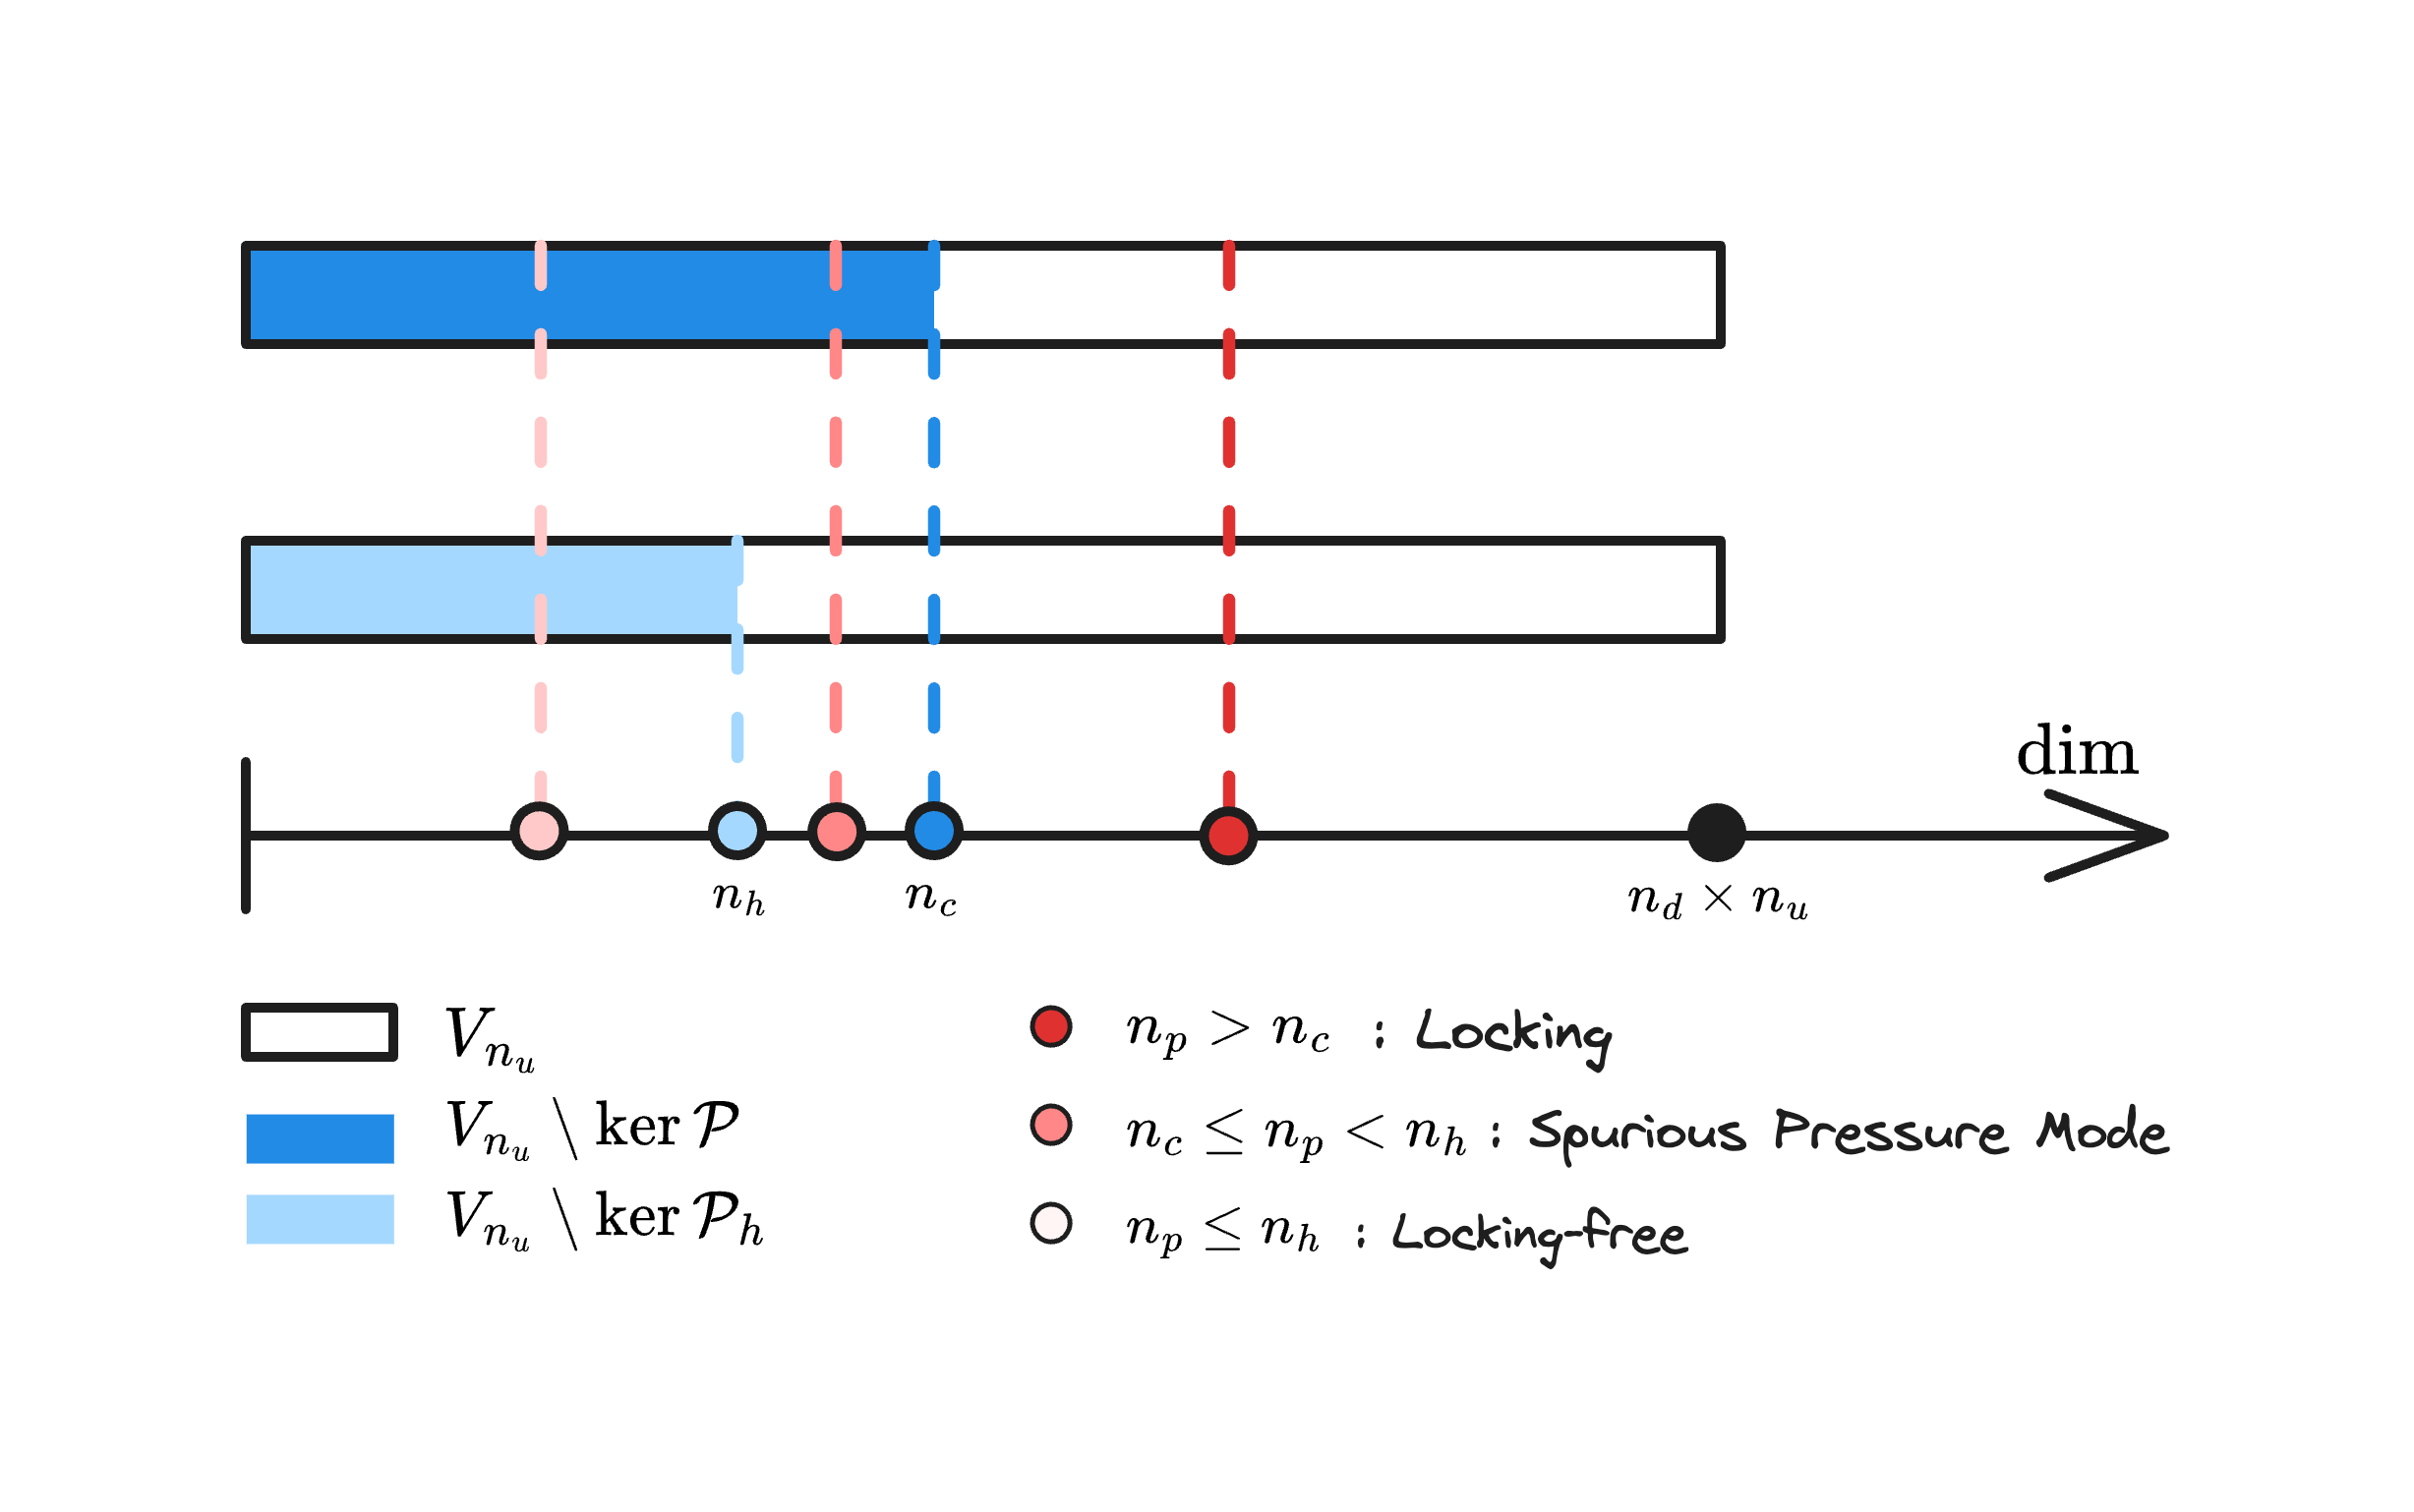
\includegraphics[width=0.8\textwidth]{png/space.png}
    \caption{Illustration of estimator}\label{fg:space}
\end{figure}
\begin{itemize}
    \item As $n_p > n_s$, there must exist a subspace in space $V_{n_u}\ker \mathcal P_h \mathcal I_h$ belong to $\ker \mathcal P$, resulting $\beta_s = 0$. At this circumstance, the LBB condition cannot be satisfied.

    \item As $n_p \le n_s$, $(V_{n_u}\setminus \ker \mathcal P_h \mathcal I_h) \subseteq (V_{n_u}\setminus \mathcal P)$, now, $\beta$ is a constant independent with $h$.
\end{itemize}

\begin{equation}
    r_{opt} \ge \frac{n_d\times n_u}{n_s} 
\end{equation}
It is worth to point that,


\subsection{Optimal volumetric constraint ratio}
From the 

\subsubsection{2D constraint ratio}
For now, $n_s$ can be considered as the optimal pressure's dofs, and the way to determine $n_c$ is shown as follows. For instance, in two dimensional nearly-incompressible elasticity problem, for linear polynomial space with dimension is 3 namely $P_3$, the counterpart displacement space $V_3$ is given by:
\begin{equation}
V_3 = \mathrm{span} \left \{
\begin{pmatrix} 1 \\ 0 \end{pmatrix},
\begin{pmatrix} 0 \\ 1 \end{pmatrix},
\begin{pmatrix} x \\ 0 \end{pmatrix},
\begin{pmatrix} 0 \\ x \end{pmatrix},
\begin{pmatrix} y \\ 0 \end{pmatrix},
\begin{pmatrix} 0 \\ y \end{pmatrix}
\right \}
\end{equation}
or rearranged as follows,
\begin{equation}\label{base1}
V_3 = \mathrm{span} 
\begin{Bmatrix}
\underbrace{
\begin{pmatrix} 1 \\ 0 \end{pmatrix},
\begin{pmatrix} 0 \\ 1 \end{pmatrix},
\begin{pmatrix} y \\ 0 \end{pmatrix},
\begin{pmatrix} 0 \\ x \end{pmatrix},
\begin{pmatrix} x \\ -y \end{pmatrix}
}_{\ker \mathcal P},
\underbrace{
\begin{pmatrix} x \\ y \end{pmatrix}
}_{V_3\setminus \ker \mathcal P}
\end{Bmatrix}
\end{equation}
It can be found from Eq. \eqref{base1}, for $n_u = 3$, $n_s = 1$. Following the path, the displacement space with quadratic polynomial base namely $V_6$ can be stated as:
\begin{equation}\label{base2}
V_6 = \mathrm{span}
\begin{Bmatrix}
\overbrace{
\begin{pmatrix} 1 \\ 0 \end{pmatrix},
\begin{pmatrix} 0 \\ 1 \end{pmatrix},
\begin{pmatrix} y \\ 0 \end{pmatrix},
\begin{pmatrix} 0 \\ x \end{pmatrix},
\begin{pmatrix} x \\ -y \end{pmatrix},
\begin{pmatrix} x^2 \\ -2xy \end{pmatrix},
\begin{pmatrix} y^2 \\ 0 \end{pmatrix},
\begin{pmatrix} 0 \\ x^2 \end{pmatrix},
\begin{pmatrix} -2xy \\ y^2 \end{pmatrix}
}^{\ker \mathcal P}, \\
\underbrace{
\begin{pmatrix} x \\ y \end{pmatrix},
\begin{pmatrix} x^2 \\ 2xy \end{pmatrix},
\begin{pmatrix} 2xy \\ y^2 \end{pmatrix}
}_{V_6\setminus \ker \mathcal P}
\end{Bmatrix}
\end{equation}
In this circumstance, $n_s = 3$. As the order of polynomial space increasing, the every optimal numbers of constraint dofs for each order are listed in Table. \ref{tab:constraint}, 
in which $n$ denoted by the order of space $P_{n_u}$.
For the flexibility of usage, the relation between $n_u$ and $n_c$ is summarized as follows:
\begin{table}[ht!]
\centering
\caption{2D Degrees of freedom and volumetric constraint}
\label{tab:constraint_2D}
\begin{tabular}{ccc}
\toprule
    $n_u$ & $n$ & $n_s$ \\
\midrule
3  & 1 & 1 \\
6  & 2 & 3 \\
10 & 3 & 6 \\
15 & 4 & 10 \\
\vdots & \vdots & \vdots \\
$n_u$ & $\left \lfloor \frac{\sqrt{1+8n_u}-3}{2} \right \rfloor$ & $\frac{n(n+1)}{2}$ \\
\bottomrule
\end{tabular}
\end{table}

\begin{equation}
    r_{opt} \ge \frac{n_d\times n_u}{n_s}
    ,\quad 
    n_s = \frac{n(n + 1)}{2} 
    ,\quad
    n = \left \lfloor \frac{\sqrt{1 + 8n_u} - 3}{2} \right \rfloor 
\end{equation}

% TODO: discuss about union-jack element arrangement

\subsection{3D constraint ratio}

\begin{equation}
    V_4 = \mathrm{span} 
    \begin{Bmatrix}
        \overbrace{
            \begin{pmatrix} 1 \\ 0 \\ 0 \end{pmatrix},
            \begin{pmatrix} 0 \\ 1 \\ 0 \end{pmatrix},
            \begin{pmatrix} 0 \\ 0 \\ 1 \end{pmatrix},
            \begin{pmatrix} 0 \\ x \\ 0 \end{pmatrix},
            \begin{pmatrix} 0 \\ 0 \\ x \end{pmatrix},
            \begin{pmatrix} y \\ 0 \\ 0 \end{pmatrix}
        }^{\ker \mathcal P},
            \\
        \underbrace{
            \begin{pmatrix} 0 \\ 0 \\ y \end{pmatrix},
            \begin{pmatrix} z \\ 0 \\ 0 \end{pmatrix},
            \begin{pmatrix} 0 \\ z \\ 0 \end{pmatrix},
            \begin{pmatrix} x \\-y \\ 0 \end{pmatrix},
            \begin{pmatrix} x \\ 0 \\-z \end{pmatrix}
        }_{\ker \mathcal P}, 
        \underbrace{
            \begin{pmatrix} x \\ y \\ z \end{pmatrix}
        }_{V_{n_u}\setminus \ker \mathcal P}
    \end{Bmatrix}
\end{equation}

\begin{table}[ht!]
\centering
\caption{3D Degrees of freedom and volumetric constraint}
\label{tab:constraint_3D}
\begin{tabular}{ccc}
\toprule
    $n_u$ & $n$ & $n_s$ \\
\midrule
4  & 1 & 1 \\
10 & 2 & 4 \\
20 & 3 & 10 \\
\vdots & \vdots & \vdots \\
$n_u$ & $n$ & $\frac{n(n+1)(n+3)}{6}$ \\
\bottomrule
\end{tabular}
\end{table}

\begin{align}
    n_s &= \frac{n(n + 1)(n + 2)}{6} \\ 
    n&= 
    \left \lfloor
    \left (3n_u + \frac{1}{3}\sqrt{81n_u^2 - \frac{1}{3}} \right )^{\frac{1}{3}}
    +
    \frac{1}{
        3\left (3n_u + \frac{1}{3}\sqrt{81n_u^2 - \frac{1}{3}} \right )^{\frac{1}{3}}
    } - 2
    \right \rfloor
\end{align}

